\documentclass[11pt, letterpaper]{article}

% ---------- packages ----------
\usepackage[margin=0.7in]{geometry}
\usepackage{tcolorbox}
\usepackage{enumitem}
\usepackage{hyperref}
\usepackage{xcolor}
\usepackage{titlesec}
\usepackage{fancyhdr}
\usepackage{graphicx}
\usepackage{tabularx}
\usepackage{booktabs}

% ---------- colors ----------
\definecolor{boxborder}{RGB}{60, 90, 150}
\definecolor{boxbg}{RGB}{245, 248, 255}
\definecolor{headcolor}{HTML}{00636f}
\definecolor{placeholder}{RGB}{140, 140, 140}

% ---------- tcolorbox style ----------
\tcbset{
  sectionbox/.style={
    colframe=boxborder,
    colback=boxbg,
    boxrule=0.6pt,
    arc=2pt,
    left=6pt, right=6pt, top=4pt, bottom=4pt,
    fontupper=\scriptsize,
  }
}

% ---------- placeholder command ----------
\newcommand{\placeholder}[1]{\textcolor{placeholder}{\textit{#1}}}

% ---------- section formatting ----------
\titleformat{\section}
  {\normalsize\bfseries\color{headcolor}}{\thesection.}{0.4em}{}
\titlespacing*{\section}{0pt}{6pt}{2pt}

% ---------- header / footer ----------
\pagestyle{fancy}
\fancyhf{}
\renewcommand{\headrulewidth}{0.4pt}
\lhead{\small\color{headcolor} CS 4100 -- Project Executive Summary}
\cfoot{\small\thepage}

% ---------- suppress paragraph indent ----------
\setlength{\parindent}{0pt}
\setlength{\parskip}{3pt}

\begin{document}

% ===== TITLE BLOCK =====
\begin{center}
  {\Large\bfseries\color{headcolor} PhysioPose: Real-Time Squat Form Classification from a Standard Webcam}\\[4pt]
  {\normalsize Kanishk Kaushal, Kaushal Jha}\\[2pt]
\end{center}

\vspace{4pt}

% ===== 1. MOTIVATION & PROBLEM STATEMENT =====
\section{Motivation \& Problem Statement}

Home-based physiotherapy and strength rehabilitation depend on patients
performing exercises with correct form, yet most rehabilitation happens
unsupervised, where poor technique reduces effectiveness and can cause
re-injury. The squat is one of the most prescribed lower-limb rehabilitation
and strengthening movements, but common faults---excessive forward/back lean
and lifting the heels---are easy to make and hard for an untrained person to
self-detect. Clinical motion-capture systems and wearable sensors can provide
feedback, but they are expensive, require setup, and are inaccessible for
everyday at-home use. There is a clear gap for a low-cost tool that gives
immediate form feedback using only hardware the user already owns: a webcam.
Our engineering goal is to build a system that classifies squat form in real
time from a single RGB webcam and tells the user whether their form is good or
which specific fault they are making. We build on Google's MediaPipe Pose,
which made robust on-device 2D human-pose estimation widely available~[1], and
on prior work showing joint-angle features are strong predictors of exercise
quality~[3]. The result is intended to make rehabilitation feedback more
accessible and affordable without any specialized hardware.

% ===== 2. APPROACH =====
\section{Approach}

PhysioPose is a real-time pipeline: each webcam frame is passed to MediaPipe
Pose, which returns 33 body landmarks; we then convert the relevant landmarks
into a small set of biomechanical features and classify the current posture.
Rather than feeding raw pixel coordinates to the model, we compute four
\emph{resolution-invariant joint angles}---knee, hip, ankle, and spine (torso)
angle---using vector geometry between landmark triples. These angles capture
exactly the cues a physiotherapist watches: knee/hip angle for squat depth,
spine angle for torso lean (the ``bad back'' fault), and ankle angle for heel
lift (the ``bad heel'' fault). The features are fed to a Random Forest
classifier (scikit-learn, 200 trees, balanced class weights) that outputs one
of three labels---\textbf{Good form}, \textbf{Bad back}, or \textbf{Bad
heel}---with a confidence score that is overlaid live on the video. We trained
on a public side-view squat image dataset (Zenodo~[2], $\sim$3{,}800 images),
running every image through the \emph{same} MediaPipe + angle-extraction code
used at inference so that training and live features are produced identically.
The primary tools are Python~3.10, OpenCV (capture/overlay), MediaPipe Pose
(landmarks), and scikit-learn/pandas (features and model). Key design decisions
were (i) using angle features instead of pixel coordinates for camera- and
resolution-independence, and (ii) extracting from the single camera-facing leg
so that side-view occlusion of the far leg does not discard frames. Scope and
assumptions: the user stands side-on, full body in frame, one person, and we
classify a fixed set of three squat faults rather than arbitrary exercises.

% ===== 3. KEY RESULTS =====
\section{Key Results}

On a held-out test split of the Zenodo benchmark, the Random Forest reaches
\textbf{87\% accuracy} across the three classes (left). Performance is strongest
on \textbf{Bad back}, with \textbf{1.00 precision} and 0.88 recall---torso lean
is a clean, well-separated signal, which the feature-importance chart (right)
confirms: the spine angle is the single most informative feature, followed by
the ankle angle that drives heel detection. The dominant error is Good-vs-Bad
heel confusion (78 of 310 ``Good'' test frames are read as ``Bad heel''),
because the difference between a slightly raised heel and a flat foot is small
and noisy in 2D. The most important practical finding was a \emph{domain-shift}
effect: a model trained on the high-resolution benchmark photos degraded
sharply on our own 480p webcam, where joint angles read systematically
$15$--$20^{\circ}$ higher. Retraining on a small set of self-recorded webcam
squats brought the system in-domain and made live prediction usable, though
with limited recorded data ($\sim$1{,}000 frames) in-domain accuracy was lower
($\sim$63\%), again with Good/Bad-heel as the hard pair. This matched our
expectation that feature \emph{parity} between training and inference matters
more than raw dataset size, and it cleanly separates the two faults that are
geometrically distinct (lean, heel) from the harder near-threshold cases.
\vspace{-2pt}

\vspace{-2pt}
\begin{center}
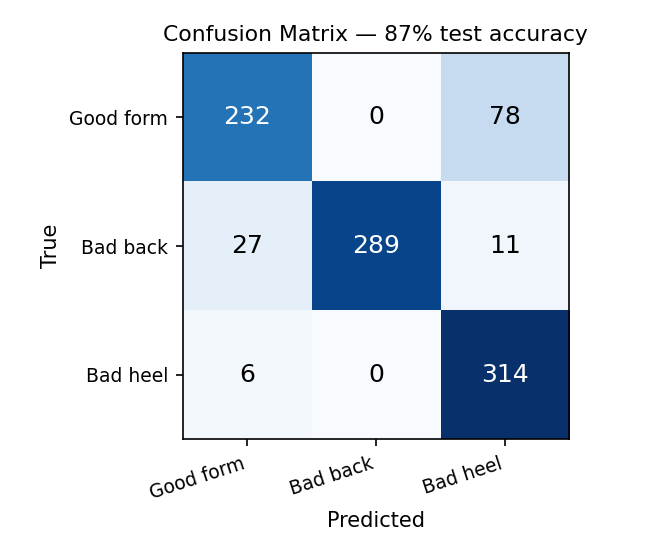
\includegraphics[width=0.40\linewidth]{confusion_matrix.png}\hspace{2em}
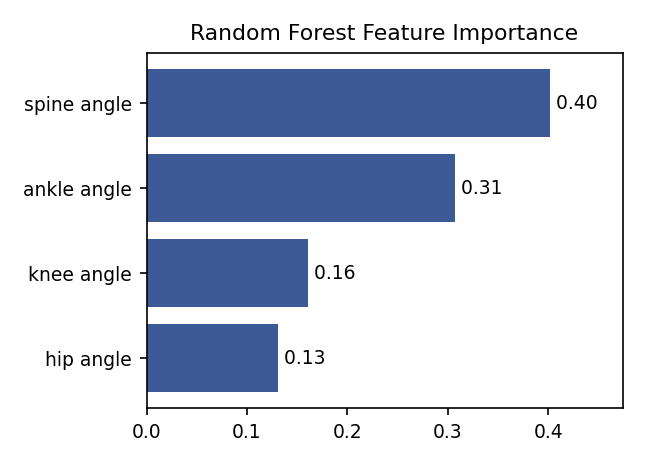
\includegraphics[width=0.37\linewidth]{feature_importance.png}
\end{center}
\vspace{-4pt}

% ===== 4. CHALLENGES & LESSONS LEARNED =====
\section{Challenges \& Lessons Learned}

Our first dataset was synthetic---``bad'' squats were generated by adding noise
to correct ones---and the resulting model collapsed to predicting a single
class regardless of input; it could not even recover its own training-class
means. The lesson was to validate a model against its own data distribution
before trusting accuracy numbers, and that realistic data beats synthetic
perturbations. The second major issue was a train/inference mismatch: features
computed in raw pixels (e.g.\ hip depth) were $\sim$7$\times$ larger on the
3456\,px training images than on the 480p webcam, so the model keyed on splits
that could never fire live---we fixed this by switching to scale-invariant
angle features. Side-view occlusion of the far leg initially discarded most
frames, which we solved by extracting features from the single visible leg and
relaxing the landmark-visibility threshold. Finally, the photo-to-webcam domain
gap forced us to record our own calibration data on the target camera. The
overarching lesson: in a perception pipeline, guaranteeing that training and
live features come from the identical code path is as important as the model
itself.

% ===== 5. INDIVIDUAL CONTRIBUTIONS =====
\section{Individual Contributions}
\begin{tcolorbox}[sectionbox, height=2.6cm, valign=top]
  \vspace{2pt}
  \centering
  \begin{tabularx}{0.95\textwidth}{l X c}
    \toprule
    \textbf{Member} & \textbf{Primary Contributions} & \textbf{Approx.\ \%} \\
    \midrule
    Kanishk Kaushal & Feature extraction, ML training/evaluation, dataset pipeline, domain-shift debugging, live integration, and documentation; plus shared foundational work below & 75\% \\
    Kaushal Jha & Repository setup, dependency configuration, webcam capture pipeline, pose-estimation integration, and dataset sourcing (jointly with Kanishk) & 25\% \\
    \bottomrule
  \end{tabularx}
\end{tcolorbox}

% ===== 6. REPOSITORY & REFERENCES =====
\section{Repository \& References}
\begin{tcolorbox}[sectionbox, height=4.2cm, valign=top]
  \textbf{GitHub Repository:}
  \href{https://github.com/Kanishk-Kaushal/PhysioPose}%
       {\texttt{https://github.com/Kanishk-Kaushal/PhysioPose}}\\[2pt]
  \textbf{Project Tracker:}
  \href{https://github.com/users/Kanishk-Kaushal/projects/3/views/1}%
       {\texttt{https://github.com/users/Kanishk-Kaushal/projects/3/views/1}}\\[2pt]
  \placeholder{Ensure the repo is public, or add the instructor as a collaborator.}

  \vspace{6pt}
  \textbf{Key References:}
  \begin{enumerate}[leftmargin=1.4em, itemsep=1pt, topsep=2pt, label={[\arabic*]}]
    \item C.\ Lugaresi et al., ``MediaPipe: A Framework for Building Perception
      Pipelines,'' Google Research, 2019. Real-time on-device 2D pose
      estimation used for landmark detection.
    \item C.\ Teng, ``Squat Posture Image Dataset (Good / Bad Back / Bad
      Heel),'' Zenodo, 2025, record 17558630. Side-view labeled images used for
      training and benchmarking.
    \item D.\ R.\ Beddiar et al., ``Vision-based human activity recognition for
      rehabilitation,'' (survey context for pose-based exercise assessment).
  \end{enumerate}
\end{tcolorbox}

\end{document}
